
\subsection{Processor Model}
\begin{figure}[t]
\centering
%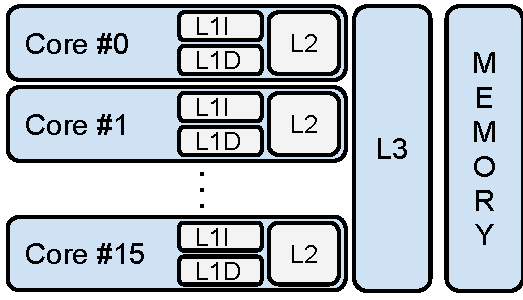
\includegraphics[scale=.65]{figures/processor_model}
\caption{Processor model architecture.}
\label{fig:processor_model}
\end{figure}


\begin{table}[ht]
\centering
\begin{tabular}{rl}
\toprule
\bf{Processor core}                 & 3GHz, OOO, 6 inst. dispatch width,     \\
                                    & 128 rob entries, 4 inst. commit width, \\
                                    & 3 Int. ALU, 1 FP MUL/DIV, 1 FP ADD, \\
                                    & 2 Int. SSE ALU, 1 Int. SSE MUL \\
\bf{Private L1 inst.}               & 32kB, 64B block-size, 4-way, 8 MSHRs, \\
									& LRU, Tag/Data 1/1 cycles \\
\bf{Private L1 data}                & 32kB, 64B block-size, 8-way, 8 MSHRs, \\
									& LRU, Tag/Data 1/2 cycles \\
\bf{Private L2 unified cache}       & 128kB, 64B block-size, 8-way, \\
                                    & 12 MSHRs, LRU, Tag/Data 1/2 cycles     \\
\bf{Shared L3 cache}                & 4/8/16MB, 64B block-size, 24 MSHRs, \\
                                    & 32-way, varying replacement algorithm \\
                                    & Tag/Data 2/5, 2/6, 3/7, 3/9 cycles         \\
\bf{Memory controller}              & 6.4GB/s, 100ns access latency         \\
\bf{Clock Skew}                     & 100 cycle barrier synchronization        \\
\bottomrule                             
\end{tabular}
\caption{Model properties.}
\label{tbl:processor_model:properties}
\end{table}

In this paper, we model a CMP model with two levels of private cache and a shared third layer.
This model is simulated using the Sniper~\cite{Carlson2011} simulation system.
An overview of the system is shown in Figure~\ref{fig:processor_model}, and Table~\ref{tbl:processor_model:properties} lists the system properties.

We are using the Nehalem core model in Sniper and have selected our processor core properties and first level cache size based on the original Intel Nehalem~\cite{Thomadakis2011}. 
We do note that in more recent architectures such as Intel's Haswell~\cite{Jain2013} the core properties have changed compared to the older Nehalem, but the size of the first level cache remains the same.
The reason being that with increasing cache size the access latency increases making it cache unable to feed the processor pipeline with a sufficient stream of instructions and data.

For 4-, 8- and 16-core simulations we will respectively use a 4MB, 8MB, and 16MB L3 configuration.
CACTI~\cite{cacti4} is used to estimate cache latencies for all cache levels.
We configure CACTI to use high-performance storage cells and optimize towards lower access latencies.

\subsection{Benchmarks and Workloads}
\label{sec:methodology:benchmarks}
In all our experiments, we are utilizing benchmarks from the SPEC CPU2006~\cite{spec2006} benchmark suite. 
We use SimPoint~\cite{simpoint30} to extract 250M instruction intervals from each benchmark that we use in all experiments.
By only extracting a single interval we are willingly increasing the error~\cite{Hamerly2004} between our interval and the results obtained by simulating the entire benchmark.
In our experiments, we are interested in observing performance change in our simulated intervals due to architectural changes.
Producing results comparable to the results of the full benchmark run is not required to achieve this.
Also, it is not obvious how to correctly combine performance metrics used in this thesis from multiple simulated intervals.
Therefore, we choose to use only one interval per benchmark.

We classify each interval based on its sensitivity to changes in available cache space and memory bandwidth.
Based on these classifications we group all benchmarks into one of the following groups:
\begin{itemize}
\item \textbf{Cache sensitive} (ca) benchmarks are in general benchmarks with memory access patterns that are recency-friendly. 

\item \textbf{Bandwidth sensitive} (bw) are benchmarks with no to little temporal locality, often streaming access patterns. 

\item \textbf{Cache- and Bandwidth sensitive} (cabw) are benchmarks with trashing memory access patterns that will benefit from more cache (less trashing) and more bandwidth (faster loading of previously trashed data).

\item \textbf{Compute sensitive} (co) are benchmarks limited by the processing power of the simulated processor.
\end{itemize}
Based on these classifications we generated 4, 8 and 16 core workloads.
The 4 core workloads come in five classes.
One class per benchmark group, these contain workloads only from that particular group.
Also, one class with benchmarks picked from all groups.
The ca and cabw groups contain 5 workloads while the bw and co groups contain 10 workloads.
There is only a single class of 8 and 16 core workloads, as there are not enough benchmarks per group to make workloads of this size. 
The ten 8 and 16 core workloads contain benchmarks from across all benchmark groups.

\subsection{Metrics}
\label{sec:methodology:metrics}
We utilize two metrics to measure the effect of destructive interference between benchmarks in multicore simulations.
System Throughput (STP)~\cite{Eeckhout2010} and the Hamonic Mean of Speedups (HMS)~\cite{Eeckhout2010}.

Two concepts are needed to define these metrics; private mode execution time and shared mode execution time.
Shared mode execution time is the simulation time of a benchmark when run as a part of a workload.
Private mode execution time is the simulation time of a benchmark when run alone on the same processor model.
By definition, we expect a benchmark to execute slower in shared mode than in private mode.

Based on private and shared mode execution time we can define Normalized Progress (NP), or speedup, as ${NP}_i = \frac{T^{P}_i}{T^{S}_i}$.
Here $T^{P}_i$ and $T^{S}_i$ is respectively the private and shared mode execution time for benchmark $i$.
Normalized progress is a measure of benchmark progression in shared mode.
STP is defined by L. Eeckhout~\cite{Eeckhout2010} as the sum of NP for all benchmarks in a workload, as shown in Equation~\ref{eq:STP}.

\begin{equation} \label{eq:STP} 
 {STP} = {\sum\limits_{n=1}^{k}}\frac{T^{P}_i}{T^{S}_i}
\end{equation}

We also define HMS as the harmonic mean of NP values, as shown in Equation~\ref{eq:HMS}.
The summation kernel in HMS is also known as Normalized Turnaround Time (NTT).
HMS is therefore by definition the reciprocal of Average Normalized Turnaround Time (ANTT)~\cite{Eeckhout2010}, and hence HMS has a system level meaning relating to the benchmark's average normalized turnaround-time.

\begin{equation} \label{eq:HMS}
 {HMS} = \frac{k}{{\sum\limits_{n=1}^{k}\frac{1}{\frac{T^{P}_i}{T^{S}_i}}}} = \frac{k}{{\sum\limits_{n=1}^{k}\frac{T^{S}_i}{T^{P}_i}}}
\end{equation}

Finally, we measure cache misses per kilo instruction, MPKI, for all experiments.